\documentclass[a4paper]{article}
\usepackage[14pt]{extsizes} % для того чтобы задать нестандартный 14-ый размер шрифта
\usepackage[utf8]{inputenc}
\usepackage[english, russian]{babel}
\usepackage{setspace,amsmath}
\usepackage{epigraph} % для эпиграфов и продвинутых цитат
\usepackage{csquotes} % ещё одна штука для цитат
\usepackage[unicode, pdftex]{hyperref} % подключаем hyperref (для ссылок внутри  pdf)
\hypersetup{
    colorlinks,
    citecolor=black,
    filecolor=black,
    linkcolor=black,
    urlcolor=black
}
\usepackage{amssymb} % в том числе для красивого знака пустого множества
\usepackage{amsthm} % в т.ч. для оформления доказательств
\usepackage[left=20mm, top=15mm, right=15mm, bottom=15mm, footskip=7mm]{geometry} % настройки полей документа 
\usepackage[active]{srcltx}
\usepackage{indentfirst}
\usepackage{listings}
\usepackage{tocloft}
\usepackage{misccorr} 
\usepackage{graphicx}
\usepackage{caption}
\usepackage[style=numeric,sorting=none]{biblatex}
\DeclareCaptionLabelSeparator{defffis}{ --- }
\captionsetup{justification=centering,labelsep=defffis}
\graphicspath{{images/}}
\DeclareGraphicsExtensions{.jpg}
\renewcommand{\cftsecleader}{\cftdotfill{\cftsubsecdotsep}}
\newcommand{\ran}{{\rm ran}\,}
\newcommand{\diag}{{\rm diag}\,}
% переименовываем  список литературы в "список используемой литературы"
\addto\captionsrussian{\def\refname{Список используемой литературы}}
\addto\captionsrussian{\renewcommand\listfigurename{Список рисунков}}
\newcounter{totreferences}
\pretocmd{\bibitem}{\addtocounter{totreferences}{1}}{}{}
\newtheorem{theorem}{Теорема} % задаём выводимое слово (для теорем)
\newtheorem{definition}{Опредление} % задаём выводимое слово (для определений) 
% объявляем новые команды 
\newcommand{\RNumb}[1]{\uppercase\expandafter{\romannumeral #1\relax}}

\begin{document} % начало документа
\def\figurename{Рисунок}

\makeatletter
\lst@UserCommand\lstlistlistingname{Список листингов кода:}
\makeatother
 
\begin{center}
\large{\textbf{SCREEN CHANGER}}\\
Версия 2.0\\
\end{center}
\thispagestyle{empty} 
	\addcontentsline{toc}{section}{Содержание} 
    \tableofcontents % Вывод содержания
\newpage

\section{Назначение и описание программы}

Программа предназначена для упрощения работы с многомониторными конфигурациями при медленной скорости движения курсора мыши. Нажатиями горячих клавиш она позволяется переключаться на центр следующего по часовой стрелке монитора.

\section{Интерфейс программы и начало работы}

Интерфейс программы представляет собой одно окно, в котором собраны все необходимые настройки и элементы управления. На рисунках ~\ref{fig:image1} и ~\ref{fig:image2} показаны внешний вид приложения на разных системах.

\begin{figure}[h]
\center{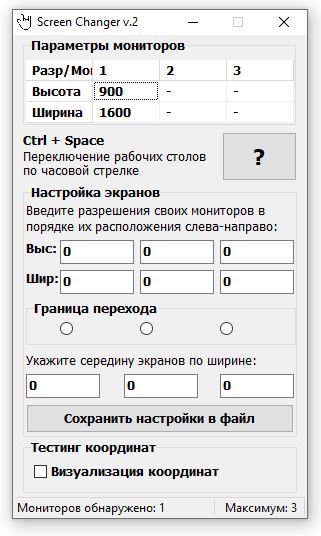
\includegraphics{001}}
\caption{Главная страница приложения}
\label{fig:image1}
\end{figure}

\begin{figure}[h]
\center{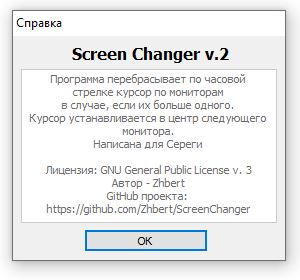
\includegraphics{002}}
\caption{Главная страница приложения на мобильном устройстве}
\label{fig:image2}
\end{figure}

\newpage
\section{Настройка утилиты}

В верхнем окне \textbf{"Параметры мониторов"} показаны автоматически найденные мониторы, подключенные к ПК. Так как в системе и в реальности расположение мониторов не всегда соответствуют друг другу, в секции \textbf{"Настройка экранов"} нужно указать разрешения экранв в том порядке, в котором они установлены физически слева-направо.

При "расширении" рабочего стола не несколько экранов обычно общее разрешение всего пространства складывается из суммы всех трех мониторов, но при этом оно не всегда находится в положительном диапазоне. Например, у вас есть два монитора, при этом левый будет иметь разрешение в отрицательном диапазоне, а правый в положительном. Условно можно сказать, что между двумя мониторами проходит граница перехода разрешений из одного диапазона в другой. 

Для определения граница следует воспользоваться секцией \textbf{"Тестинг координат"}, установив в нем чекбокс "Визуализация координат". После этого наведите курсор на каждый из ваших мониторов и нажмите комбинацию клавиш \textbf{"Ctrl + Пробел"}. Будет показано окно с текущими координатами курсора.

\begin{figure}[h]
	\center{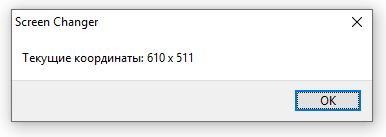
\includegraphics{003}}
	\caption{Всплывающее окно с координатами}
	\label{fig:image3}
\end{figure}

Определив таким образом полярности экранов, укажите середины каждого из них в соответствующих полях. Также нужно выбрать в секции \textbf{"Границы перехода"} место, где происходит деление полярностей мониторов. То есть, если условный ноль проходит между крайним слева и средним мониторами, следует установить средний чекбокс.

\section{Сохранение и загрузка настроек}

Для сохранения настроек нажмите клавишу \textbf{"Сохранить настройки в файл"}. Все введенные настройки будут сохранениы в конфигурационный файл \textbf{config.ini}, распложенный рядом с исполняемым файлом утилиты.

Загружаются настройки автоматически при запуске утилиты. Если конфигурационный файл не найдет, будет показано информационное окно, предупреждающее об этом.

\begin{figure}[h]
	\center{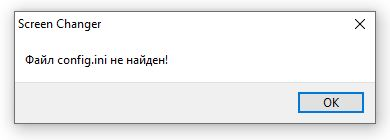
\includegraphics{004}}
	\caption{Предупреждающее окно}
	\label{fig:image4}
\end{figure}

\section{О программе}

Разработчик приложения: Нежберт Константин.

По всем вопросам и предложениям обращаться на электронную почту \\
\textbf{zhbert@yandex.ru}.

\end{document}  % КОНЕЦ ДОКУМЕНТА !